\chapter{Intelligenza Artificiale Generativa}\label{chapter:AI-generativa}

\section{Definizione di Generative AI}
La definizione di Intelligenza Artificiale Generativa si riferisce a tutte le tecniche computazionali per generare contenuto come immagini, testo, audio ed altre tipologie di dati partendo da uno specifico training data\cite{feuerriegel2024generative}.\\
Il training data è un'insieme di dati che viene utilizzato per eseguire un addestramento sul modello di rete neurale.\\
Un modello di IA Generativa è un tipo di architettura di Machine Learning che utilizza algoritmi di IA, attingendo dai pattern e dalle relazioni osservate nel training data\cite{feuerriegel2024generative}.

\section{Breve storia ed evoluzione}
L'inizio dell'ascesa dei modelli generativi può essere individuata già nei lavori di Alan Turing. Turing ha contribuito alla nascita dell'Intelligenza Artificiale attraverso il suo articolo del 1950 "\textbf{Computing Machinery and Intelligence}" \cite{turing2009computing}, introducendo il Turing Test come uno strumento che misura l'intelligenza di una macchina.
Turing ha scritto inoltre un articolo nel 1948, intitolato "\textbf{Intelligent Machinery}" \cite{turing2004intelligent} , in cui espimeva il concetto di una macchina capace di imparare dall'esperienza.
Il concetto risulta interessante perché ci permette di immaginare una macchina capace di apprendere e di essere addestrata, ponendo così le basi del Machine Learning.
Prima del 2014, tutti i modelli di deep learning esistenti, come ad esempio le Convolutional Neural Networks (CNNs)\cite{lecun1998gradient}, le Recurrent Neural Networks (RNNs)\cite{hopfield1985neural} e le Long Short-Term Memory (LSTM)\cite{hochreiter1997long}, erano principalmente descrittivi. Questi modelli miravano a spiegare i pattern nei dati e a fare previsioni basate sulle informazioni disponibili.\cite{bengesi2024advancements}\\
I GAN (Generative Adversial Network)\cite{goodfellow2020generative} hanno aperto la strada alle Generative AI. Il loro obiettivo principale è di generare nuovi campioni di dati che assomiglino strettamente ai modelli osservati nei dati di addestramento \cite{brophy2023generative}\cite{zhou2023emerging}.\\

\begin{figure}[ht]
	\centering
	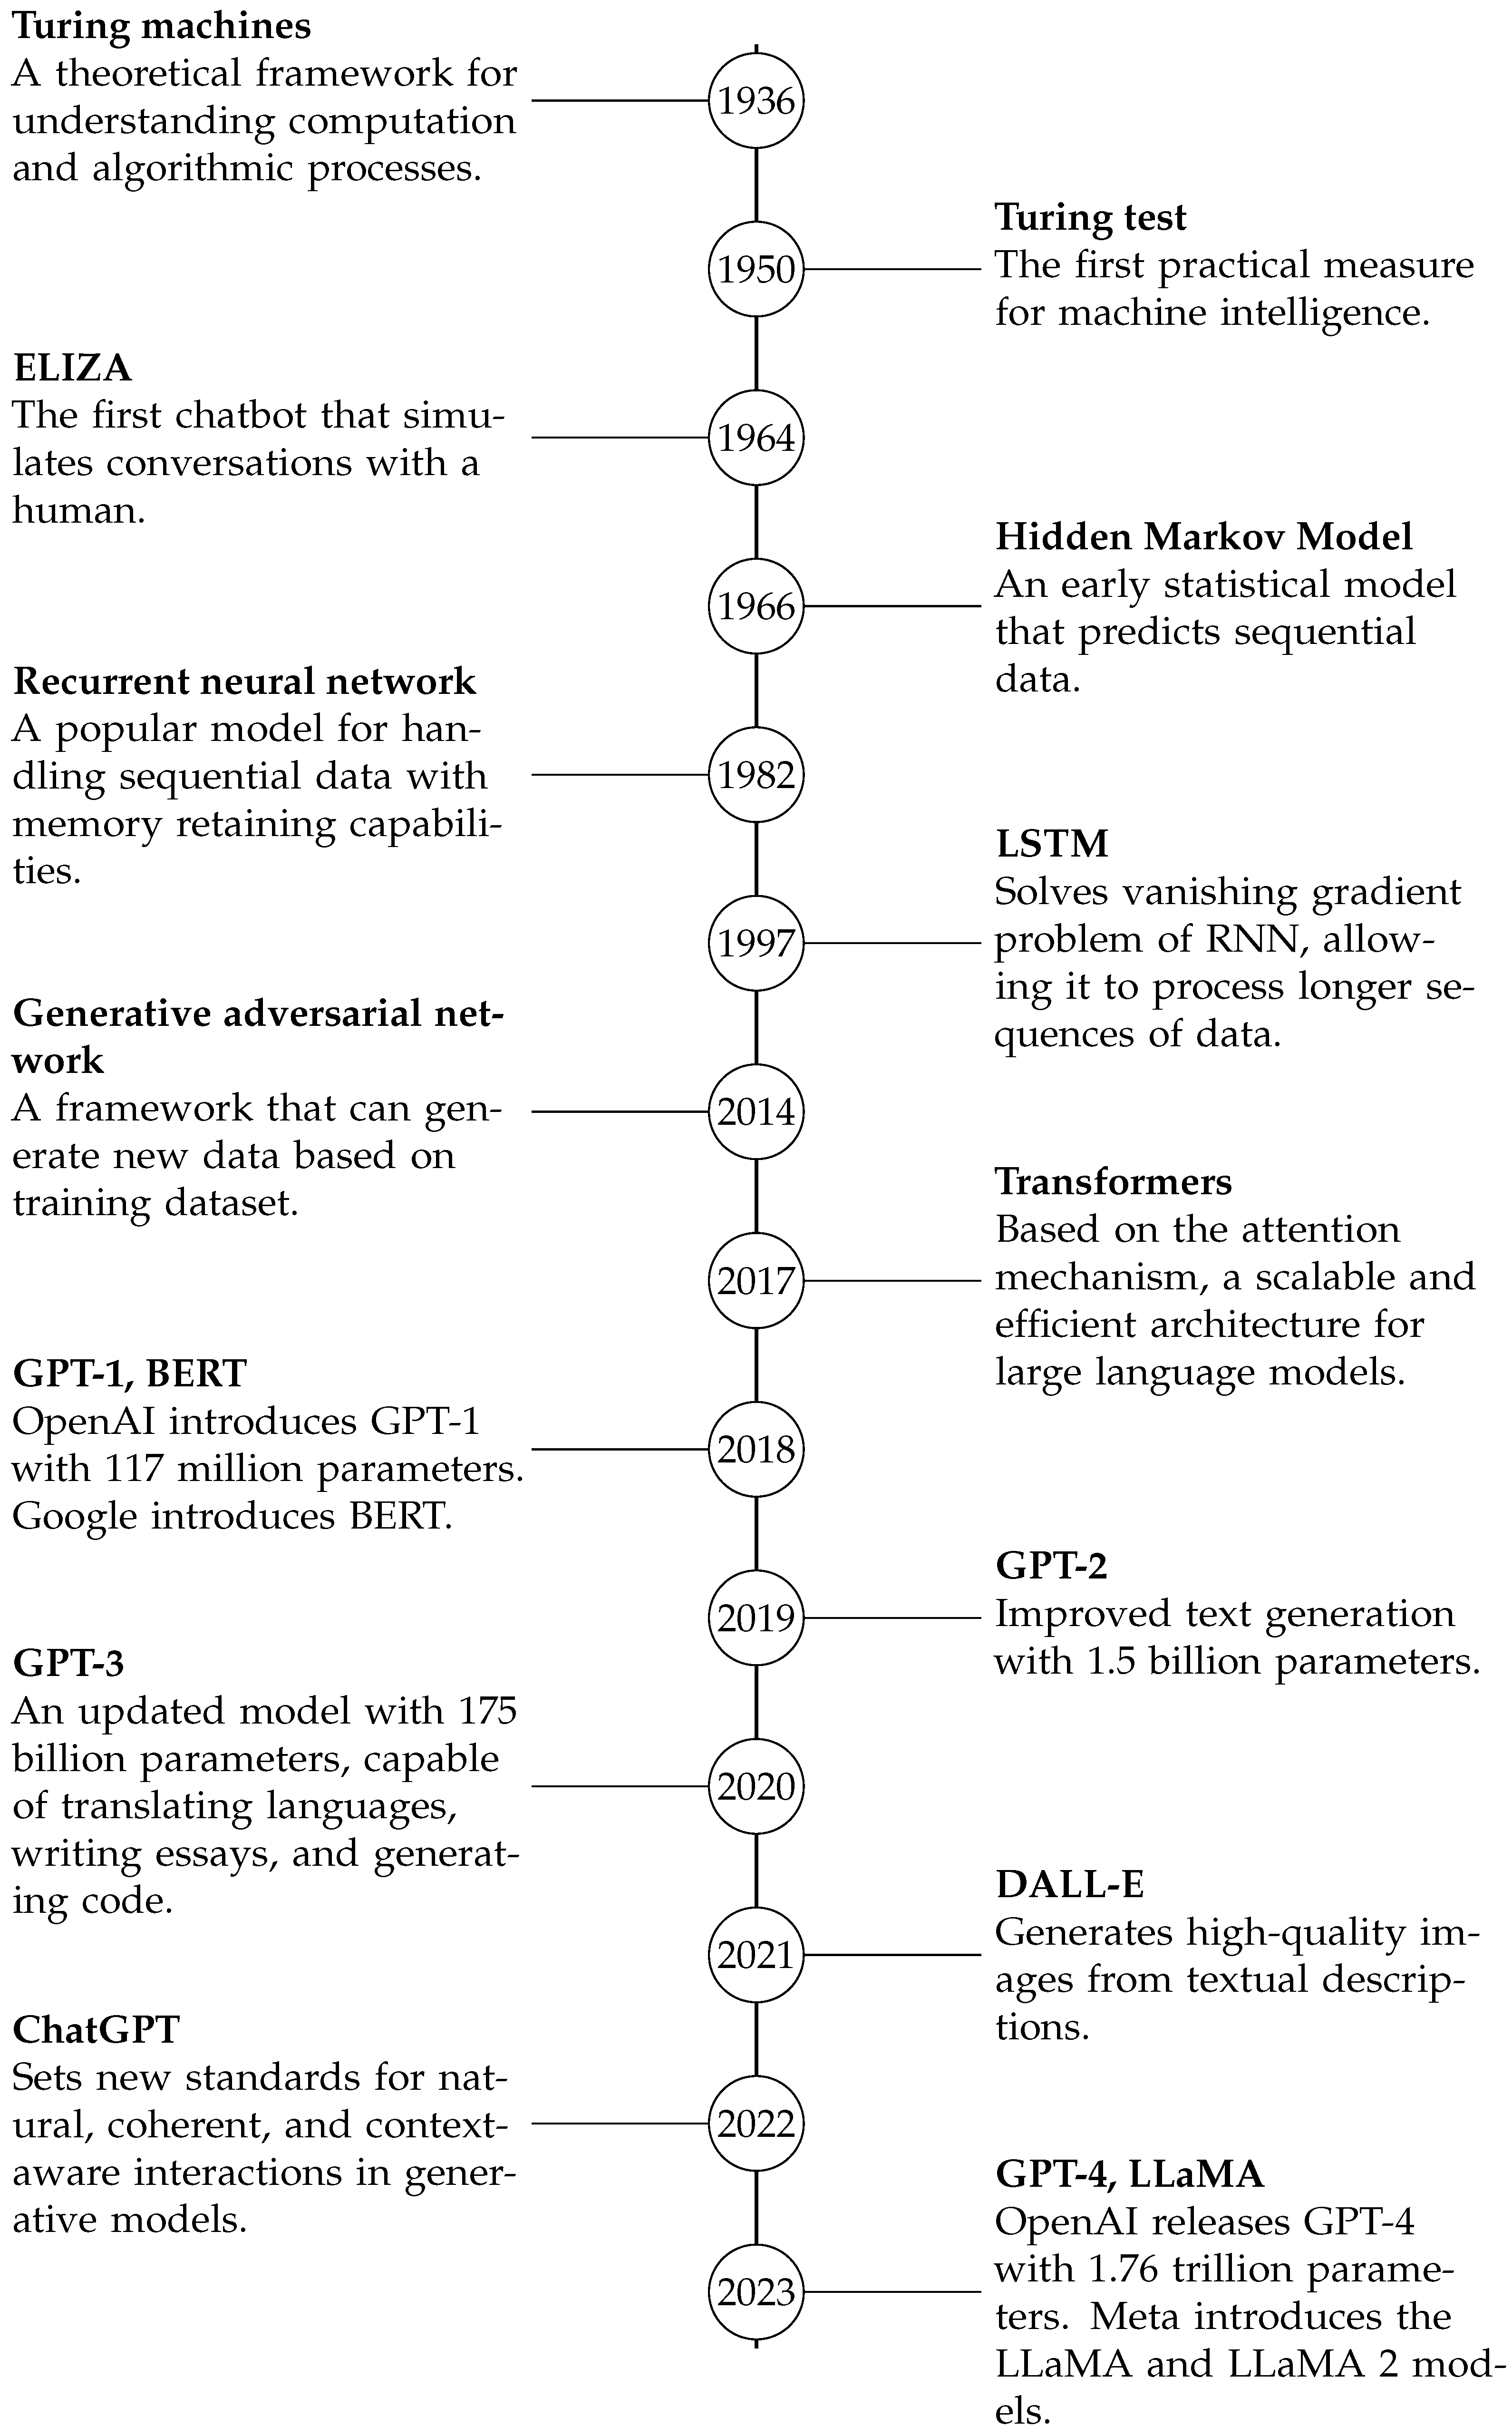
\includegraphics[width=0.3\textwidth]{Immagini/AI_story.png}
	\caption{Illustrazione della linea del tempo dello sviluppo della Generative AI, dalla Macchina di Turing fino a GPT-4 \cite{zhang2023turing}.}
	\label{fig:Generative_AI_story}
\end{figure}

\section{Generative AI sul lavoro}
Sin dalla loro introduzione intorno al 1970, i computer si sono imposti prepotentemente nel mondo del lavoro grazie alla loro capacità di eseguire in modo efficiente istruzioni pre-programmate.\\
La computerizzazione ha notevolmente ridotto i tempi di lavoro specialmente in  operazioni di routine, come l'inserimento dei dati, la contabilità e le mansioni nella catena di montaggio, determinando così una diminuzione dei posti di lavoro e  dei salari in questi settori \cite{acemoglu2011skills}.
Allo stesso tempo, questo fenomeno ha incrementato la domanda di lavoratori con abilità di programmazione, analisi dei dati e  di ricerca, portando ad un aumento della disuguaglianza salariale soprattutto negli Stati Uniti \cite{katz1992changes}.\\
In contrasto, le generative AI non richiedono specifiche istruzioni per eseguire le operazioni, ma possiedono la capacità di imparare dalle esperienze ed applicare le regole incosciamente durante il processo. Questa capacità è definita conoscenza tacita e permette di svolgere operazioni che prevedono di fare affidamento sul giudizio e sull'esperienza del modello \cite{fischer2009michael} \cite{nguyen2022empirical}.
I modelli di diffusione ed i transformers hanno avuto un grande impatto nel mondo del lavoro, trovando diverse applicazioni in vari settori grazie alla loro versatilità.

\section{Modelli di diffusione}
I modelli di diffusione sono una classe di modelli generativi che hanno lo scopo di interpretare distribuzioni di dati molto complesse.
Per ottenere uno di questi modelli si devono affrontare due fasi: la diffusione in avanti e la diffusione all'indietro.
Il primo processo serve per alterare l'architettura di distribuzione dei dati, aumentando gradualmente il livello del rumore all'interno dei dati di input fino ad ottenere un rumore gaussiano puro.
Il processo di diffusione all'indietro effettua l'operazione inversa, fornendo così un modello generativo molto flessibile e capace di generare complesse distribuzioni di dati a partire da un rumore casuale \cite{shokrollahi2023comprehensive}.\\
Per esempio, i Denoinsing, Diffusion Probabilistic Models (DDPMs) appartengono a questa classe di modelli e approssimano i parametri di un processo di diffusione utilizzando l'inferenza variazionale per produrre un'immagine di alta qualità.\cite{ho2020denoising}

\subsection{Applicazioni nell'assistenza sanitaria}
L'assistenza sanitaria è il settore in cui si sono verificati i maggiori progressi grazie all'uso dei modelli di diffusione. Le applicazioni possono includere: la ricostruzione di immagini, le traduzione di immagini e la generazione di un'immagine, tra le principali.
\subsubsection{Ricostruzione di immagini}
La \textbf{ricostruzione di immagini} è un processo di conversione di un'insieme di dati di difficile interpretazione in un'immagine target di facile comprensione.
Infatti, ottenere immagini di alta qualità è fondamentale nella immagini mediche, non solo per la riduzione dei rischi per i pazienti ma anche per l'abbassamento dei costi \cite{levac2023mri}.\\
Le normali tecniche per ricavare immagini dettagliate ed alta risoluzione prevedono alte dosi e prolungato tempo di esposizione alle radiazioni, come per esempio nel caso della Tomografia Computerizzata (CT) o la Risonanza Magnetica (MRI). Di conseguenza, sono state sviluppate strategie per ridurre l'esposizione alle radiazioni come l'uso di dosi ridotte o i processi di imaging con campionamento ridotto.
Tuttavia, queste tecniche possono ridurre il rapporto segnale-rumore (SNR) e il rapporto contrasto-rumore (CNR) influenzando la qualità finale dell'immagine. Questo problema può essere risolto applicando la ricostruzione dell'immagine \cite{shokrollahi2023comprehensive}.\\
Nel 2022 è stato introdotto un approccio chiamato MC-DDPM utilizzando il framework DDPM per raffinare la ricostruzione di immagini mediche sotto-campionate.
MC-DDPM è un approccio che potrebbe essere utilizzato anche per la ricostruzione CT e PET \cite{xie2022measurement}.\\
Nel 2023 per la ricostruzione delle immagini MRI è stata introdotta una tecnica chiamata \textbf{Adaptive Diffusion Priors} (AdaDiff).
Il metodo regola in modo dinamico i suoi priors durante la fase di inferenza per allinearsi meglio con la distribuzione dei dati di test migliorando la qualità dell'immagine \cite{gungor2023adaptive}.
\subsubsection{Traduzione di immagini}
La \textbf{traduzione da immagine ad immagine} è invece una tecnica che permette di trasformare un'immagine di un tipo in un'altra immagine di tipo diverso. Infatti, spesso, per ottenere una corretta diagnosi, dopo un CT è necessario effettuare anche un MRI, rendendo il processo più lungo e costoso.
Con l'utilizzo dei modelli di diffusione si può ridurre il tempo di esposizione grazie al miglioramento della flessibilità e della completezza dell'imaging medico.
Le due architetture fondamentali per la traduzione di immagini sono: pix2pix\cite{isola2017image} e CycleGAN\cite{chu2017cyclegan}.\\
Nel 2023 è stato impiegato un modello di diffusione chiamato SynDiff, che ha dimostrato un'elevata efficacia nella traduzione non supervisionata di immagini mediche. Dopo numerosi test, è stato dimostrato che questo metodo ottiene buoni risultati in termini di precisione, riduzione degli artefatti ed efficienza computazionale rispetto ad altri modelli. Le immagini generate risultano indistinguibili rispetto a quelle originali \cite{ozbey2023unsupervised}.
\subsubsection{Generazione di immagini}
La generazione di immagini è stata una delle prime applicazioni all'interno della sanità, soprattutto per la fabbricazione di immagini mediche artificiali 2D/3D.
Medfusion è un DDPM condizionale latente, utilizzato per la sintesi di immagini mediche. Nel lavoro di \cite{muller2023multimodal} è stata condotta un'analisi approfondita di dataset comprendenti immagini RGB del fondo oculare, scansioni CT del torace e scansioni MRI 3D del cervello di diversi soggetti. Gli autori hanno impiegato diverse metriche di valutazione della qualità delle immagini, tra cui il Peak Signal-to-Noise Ratio (PSNR), il Structural Similarity Index (SSIM) e la Fréchet Inception Distance (FID). I risultati della loro ricerca hanno dimostrato che l'approccio adottato offre una maggiore stabilità e interpretabilità, nonché una qualità superiore delle immagini rispetto ai modelli Generative Adversarial Networks.

\section{Transformers}
\subsection{Definizione di Transformers}
I Generative Transformers (GT) sono un'estensione delle reti neurali e sono designati a pesare il significato delle diverse parti di una sequenza di input, catturando le relazioni intricate tra i dati. Con un corretto addestramento ed il giusto contesto i GT possono generare ogni tipo di dato \cite{zhang2023turing}.
\subsection{Vantaggi dei Transformers rispetto alle CNNs e RNNs nell'Intelligenza Artificiale}
Questi modelli sono stati originariamente progettati per lo sviluppo del Natural Language Processing (NLP), ma successivamente sono stati adattati e applicati anche ad altri ambiti, come ad esempio la Computer Vision \cite{han2022survey}.
I transformers, grazie alla loro architettura avanzata e alla capacità di catturare relazioni a lungo raggio nei dati, presentano diversi vantaggi rispetto alle architetture CNNs ed RNNs. In primis, consentono un'elaborazione parallela dei dati e migliorano significativamente l'efficienza computazionale traducendosi in un risparmio di costi e risorse. Inoltre i GT sono in grado di raggiungere minimi locali o globali con un numero inferiore di passi di addestramento. Questo li rende particolarmente efficaci per compiti complessi come per l'elaborazione dei dati del linguaggio naturale.
A differenza delle CNNs e delle RNNs, i transformers non soffrono di problemi legati alle dipendenze a lungo raggio, un limite significativo delle RNNs, che spesso faticano a mantenere informazioni rilevanti su sequenze di dati estese. Inoltre, i transformers evitano il problema della scomparsa o dell'esplosione del gradiente, che può ostacolare il processo di apprendimento nelle reti neurali tradizionali. Questi vantaggi rendono i transformers una scelta preferibile per molte applicazioni di intelligenza artificiale, dalla traduzione automatica al riconoscimento del linguaggio \cite{vaswani2017attention}.

\subsection{Architettura del modello}
\subsubsection{Encoder-Decoder Structure}
I transformers possiedono una struttura encoder-decoder come rappresentato nella figura \ref{fig:Transformer model}.
L'encoder mappa una rappresentazione simbolica di sequenza \((x_1, \ldots, x_n)\) in una rappresentazione continua di sequenza z=\((z_1, \ldots, z_n)\).
È composto da una pila di 6 livelli identici, ognuno dei quali possiede due sottolivelli seguiti da un livello di normalizzazione.
Il primo sottolivello è il meccanismo di multi-head self-attention, mentre il secondo è una normale rete feed-forward completamente connessa.
Il decoder, dato z, genera una sequenza di simboli \((y_1, \ldots, y_n)\), un elemento per volta, che poi saranno consumati come input addizionale per la prossima generazione. La sua struttura è pressoché simile a quella dell'encoder, con ogni livello che possiede un sottolivello aggiuntivo che esegue il multi-head attention sull'output della pila dell'encoder.
Il meccanismo di self-attention viene modificato con una maschera speciale per impedire che le posizioni future possano influenzare le posizioni attuali, quindi la previsione per \(y_i\) non dipende dalle posizioni future \( y_{i+1}, y_{i+2}, \ldots \), e il contesto prevede solo i simboli già generati fino a quel punto \cite{vaswani2017attention}.

\begin{figure}[ht]
	\centering
	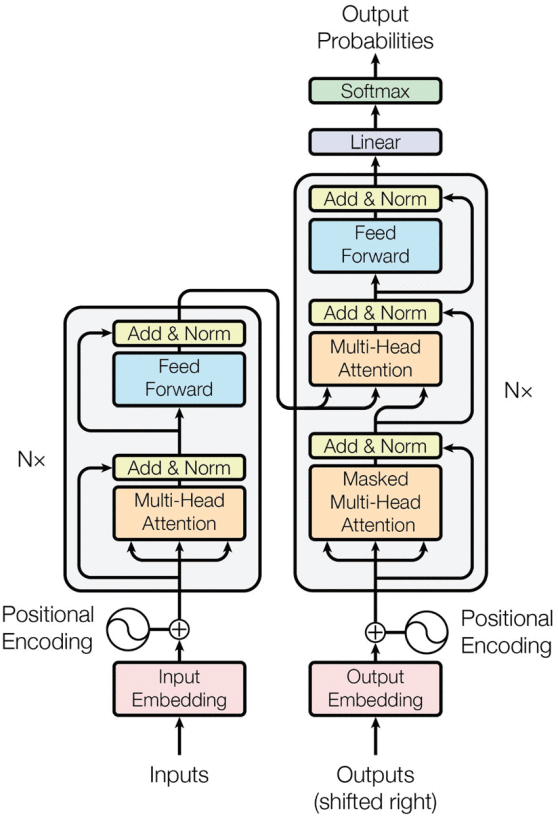
\includegraphics[width=0.3\textwidth]{Immagini/transformers.png}
	\caption{Transformer - architettura del modello \cite{vaswani2017attention}.}
	\label{fig:Transformer model}
\end{figure}

\subsubsection {Il Meccanismo Attention}
É un meccanismo che consente di capire il contesto della parola estrapolandolo dalla parte più significativa dell'input.
La funzione attention può essere rappresentata come una mappatura tra una query ed un'insieme di coppie chiave valore e l'output.
L'output è la somma pesata di tutti i valori, dove il peso di ogni valore è calcolato dalla funzione di compatibilità della query con la chiave corrispondente.
La funzione di attention permette di calcolare simultaneamente un'insieme di query, nella formula \ref{equ:attention} viene determinato l'output della funzione.

\begin{equation*} Attention(Q, K, V) = softmax\left ({{\frac {QK^{T}}{\surd d_{k}}}}\right)V \tag {6} \label{equ:attention} \end{equation*}

Dove Q rappresenta l'insieme di query, K l'insieme delle chiavi nella matrice e V l'insieme dei valori nella matrice.
Per evitare che la funzione Softmax sia indirizzata verso zone di gradiente estremamente piccole a causa di un fattore di scala molto grande, nella formula \ref{equ:attention} Il fattore di scala \(d_k\) viene sostituito con \(\frac{1}{d_k}\) \cite{vaswani2017attention}.

\begin{figure}[ht]
	\centering
	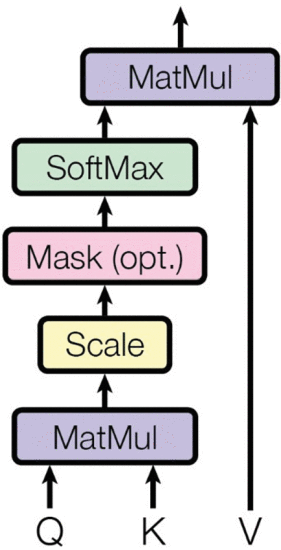
\includegraphics[width=0.3\textwidth]{Immagini/self_attention_dot.png}
	\caption{Scaled Dot-Product Attention \cite{vaswani2017attention}}
	\label{fig:Scaled Dot-Product Attention}
\end{figure}

Multi-Head Attention permette al modello di imparare diversi significati della sequenza di input, in questo modo il meccanismo di self-attention può essere eseguito molteplice volte in parallelo.
Ogni esecuzione parallela è chiamata testa. Ogni testa esplora l'input attraverso una diversa prospettiva o "sotto-spazio di rappresentazione", permettendo al modello di apprendere diverse relazioni tra gli elementi.
La formula \ref{equ:multihead_attention} mostra come gli attention output indipendenti sono concatenati e linearmente trasformati nella dimensione aspettata \cite{vaswani2017attention}.

\begin{equation*} MultiHead\left ({{ Q, K, V }}\right)=concat\left ({{ {head}_{1},\ldots {head}_{h} }}\right)W^{o} \tag {7} \label{equ:multihead_attention} \end{equation*}

dove \(\text{head}_i = \text{Attention}(QW_i^Q, KW_i^K, VW_i^V)\)

\begin{figure}[ht]
	\centering
	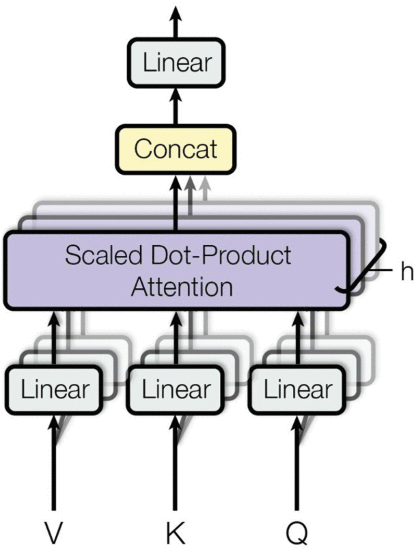
\includegraphics[width=0.3\textwidth]{Immagini/Multi-Head.png}
	\caption{ Scaled Dot-Product Multi-Head Attention \cite{vaswani2017attention}.}
	\label{fig:Multi-Head}
\end{figure}